\section{REPULSION}
\sectionsubtitle{Preventing Entry and Establishing Defensive Barriers}
\subsection{Operating Principle}
\paragraph{}{Spiritual entities respond to two forms of constraint: geometric boundaries and hierarchical authority. A closed line inscribed with names of power creates a barrier that cannot be crossed without the explicit will of the operator. This is not metaphor—the texts are precise about construction because precision matters.
}

The Solomonic system provides generalized defensive architecture. Unlike individual spirit sigils (which target specific entities of the 72), the universal divine names and geometric configurations function against the entire hierarchy. This is critical for defensive work: you establish authority over the class, not the individual.
\subsection{The Mechanism of Names}
\paragraph{}{The divine names used in Solomonic practice invoke supreme authority—not as petition, but as command. When correctly employed, these names assert the operator's position within a cosmic hierarchy that supersedes any spiritual entity being addressed.
The names function in descending order of generality:
}\begin{xltabular}{\textwidth}{|l|X|}
	\hline
	\textbf{Name} & \textbf{Function} \\ \hline
	\endfirsthead
	\hline
	\textbf{Name} & \textbf{Function} \\ \hline
	\endhead
	TETRAGRAMMATON & The four-letter name (YHVH). Supreme and unspoken authority. Commands by nature of existence itself. \\ \hline
	ADONAI & Lord. Establishes the relationship of master to subject. \\ \hline
	AGLA & Notariqon for "Atah Gibor Le-olam Adonai" (Thou art mighty forever, O Lord). Functions as protective seal. \\ \hline
	EHYEH & "I Am." Self-existent being. Cannot be questioned or countermanded. \\ \hline
	EL & God (generic). Universal divine principle. \\ \hline
	PRIMEUMATON & First moving cause. Commands origin and cessation. \\ \hline
	ANAPHAXETON & The hidden one. Binds formless and concealed entities. \\ \hline
	ON & Pure being. Existence without attribute. \\ \hline
	\caption{Universal Names of Compulsion \cite{peterson2001}}
\end{xltabular}
\paragraph{}{These names are not decorative. Each serves a specific function in the hierarchy of compulsion. TETRAGRAMMATON asserts ultimate authority. PRIMEUMATON addresses the entity's origin. ANAPHAXETON binds what attempts to hide or remain formless. When combined in the spoken formula, they create a cascading assertion of power that leaves no gap for refusal.}
\subsection{The Circle: Primary Defensive Boundary}
\paragraph{}{The Circle of Solomon serves as the operator's protected space. Its power derives from closure—a line that returns to its beginning creates a boundary without entrance. No gap, no doorway, no weakness.}
\begin{figure}[H]
	\centering
	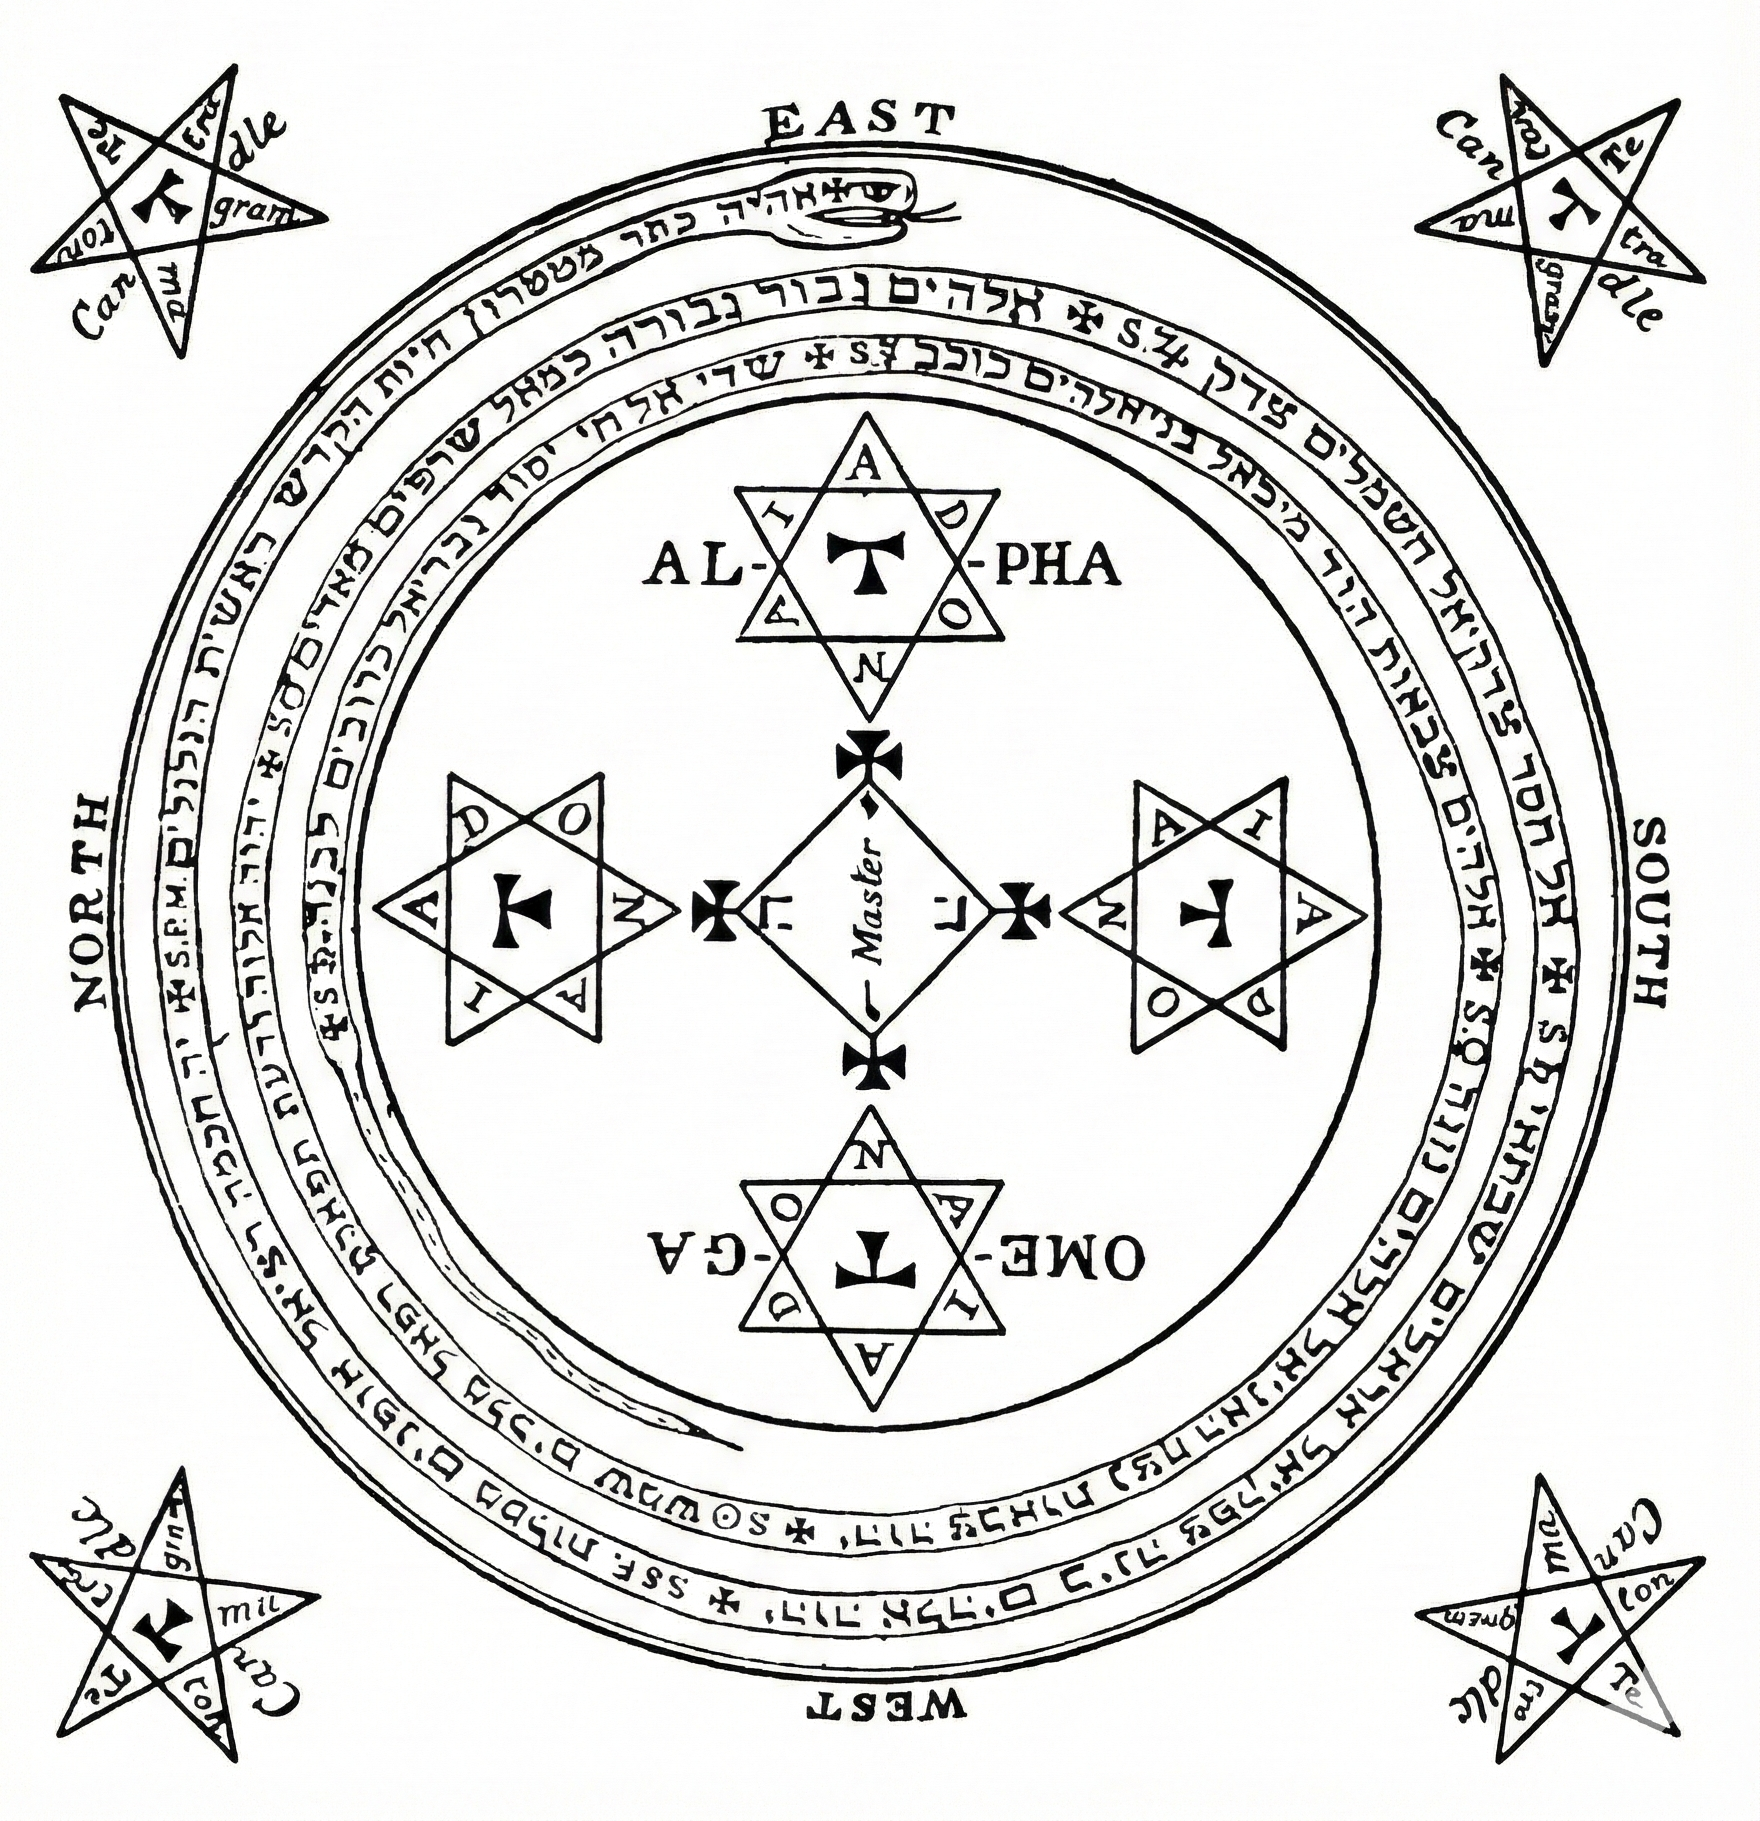
\includegraphics[width=0.3\paperwidth,keepaspectratio]{solomon_circle.png}
	\caption{The Circle of Solomon}
	\label{fig:solomoncircle}
\end{figure}
\textbf{Standard Configuration} (from the Lemegeton \textcite{peterson2001}):

\textit{Outer Ring:}
\begin{itemize}
	\item Divine name at each cardinal point (typically YHVH)
	\item Four pentagrams at North, South, East, West
	\item Tau crosses (†) between pentagrams, representing completion
	\item May include the names EHYEH, KETHER, METATRON (divine name, sephirah, archangel)
\end{itemize}
\textit{Inner Ring:}
\begin{itemize}
	\item TETRAGRAMMATON repeated at cardinal points
	\item ADONAI inscribed between
	\item Secondary divine names as needed
\end{itemize}
\textbf{Modification for Pure Defense:}

The original Solomonic circle includes a "doorway"—a deliberate gap allowing the spirit to perceive the magician during evocation. For defensive work, this gap is a liability.
Modifications:
\begin{itemize}
	\item Close all gaps. The line must be continuous.
	\item Double the boundary—inscribe two concentric circles rather than one.
	\item Add AGLA between each pentagram on the outer ring.
	\item If working in a fixed location, inscribe permanently in salt, chalk, or graved metal.
\end{itemize}

The doubled circle provides redundancy. If the outer line is compromised, the inner holds. The continuous closure prevents any entry point that could be exploited.
\subsection{The Triangle of Art: Directional Repulsion}
\paragraph{}{The Triangle serves a different function than the Circle. Where the Circle is omni-directional protection, the Triangle focuses force in a single direction. Its orientation determines its use.
}\begin{figure}[H]
	\centering
	\includegraphics[width=0.3\paperwidth,keepaspectratio]{solomon_triangle.png}
	\caption{The Triangle of Art}
	\label{fig:solomontriangle}
\end{figure}
\textbf{Repulsion Configuration:}

Point the apex OUTWARD from the space being protected. This creates a geometric wedge that drives force away from the protected area toward the triangle's point.
Inscribe on the three sides:
\begin{itemize}
	\item PRIMEUMATON (the first mover—commands beginning and end)
	\item ANAPHAXETON (the hidden one—binds formless entities)
	\item TETRAGRAMMATON (supreme name—ultimate authority)
\end{itemize}

Place MI-CHA-EL at the three points of the triangle. Michael is the specific archangelic force associated with the expulsion of rebellious spirits. His name at each vertex channels that function through the geometric form.

At the center of the triangle, inscribe the Hexagram of Solomon (see below) with no specific entity's sigil inside. The empty hexagram functions as a universal binding symbol—it affects any entity without requiring specific identification.
\begin{figure}[H]
	\centering
	\includegraphics[width=0.3\paperwidth,keepaspectratio]{solomon_hexagram.png}
	\caption{The Hexagram of Solomon}
	\label{fig:solomonhexagram}
	\cite{peterson2001}
\end{figure}
\textbf{Deployment:}

Place the repulsion triangle at thresholds, windows, or any point of suspected entry. The point faces outward—toward the direction of approach. For a room with multiple access points, multiple triangles may be required.

The triangle does not create an impassable barrier like the circle. It creates resistance and discomfort. An entity approaching a correctly configured triangle will experience increasing difficulty as it nears. This makes it ideal for areas where complete sealing is impractical but deterrence is needed.
\subsection{The Pentagram of Solomon}
\paragraph{}{The pentagram is the most versatile generalized symbol in the Solomonic system. Unlike the circle (which protects a space) or the triangle (which directs force), the pentagram protects the person.}
\begin{figure}[H]
	\centering
	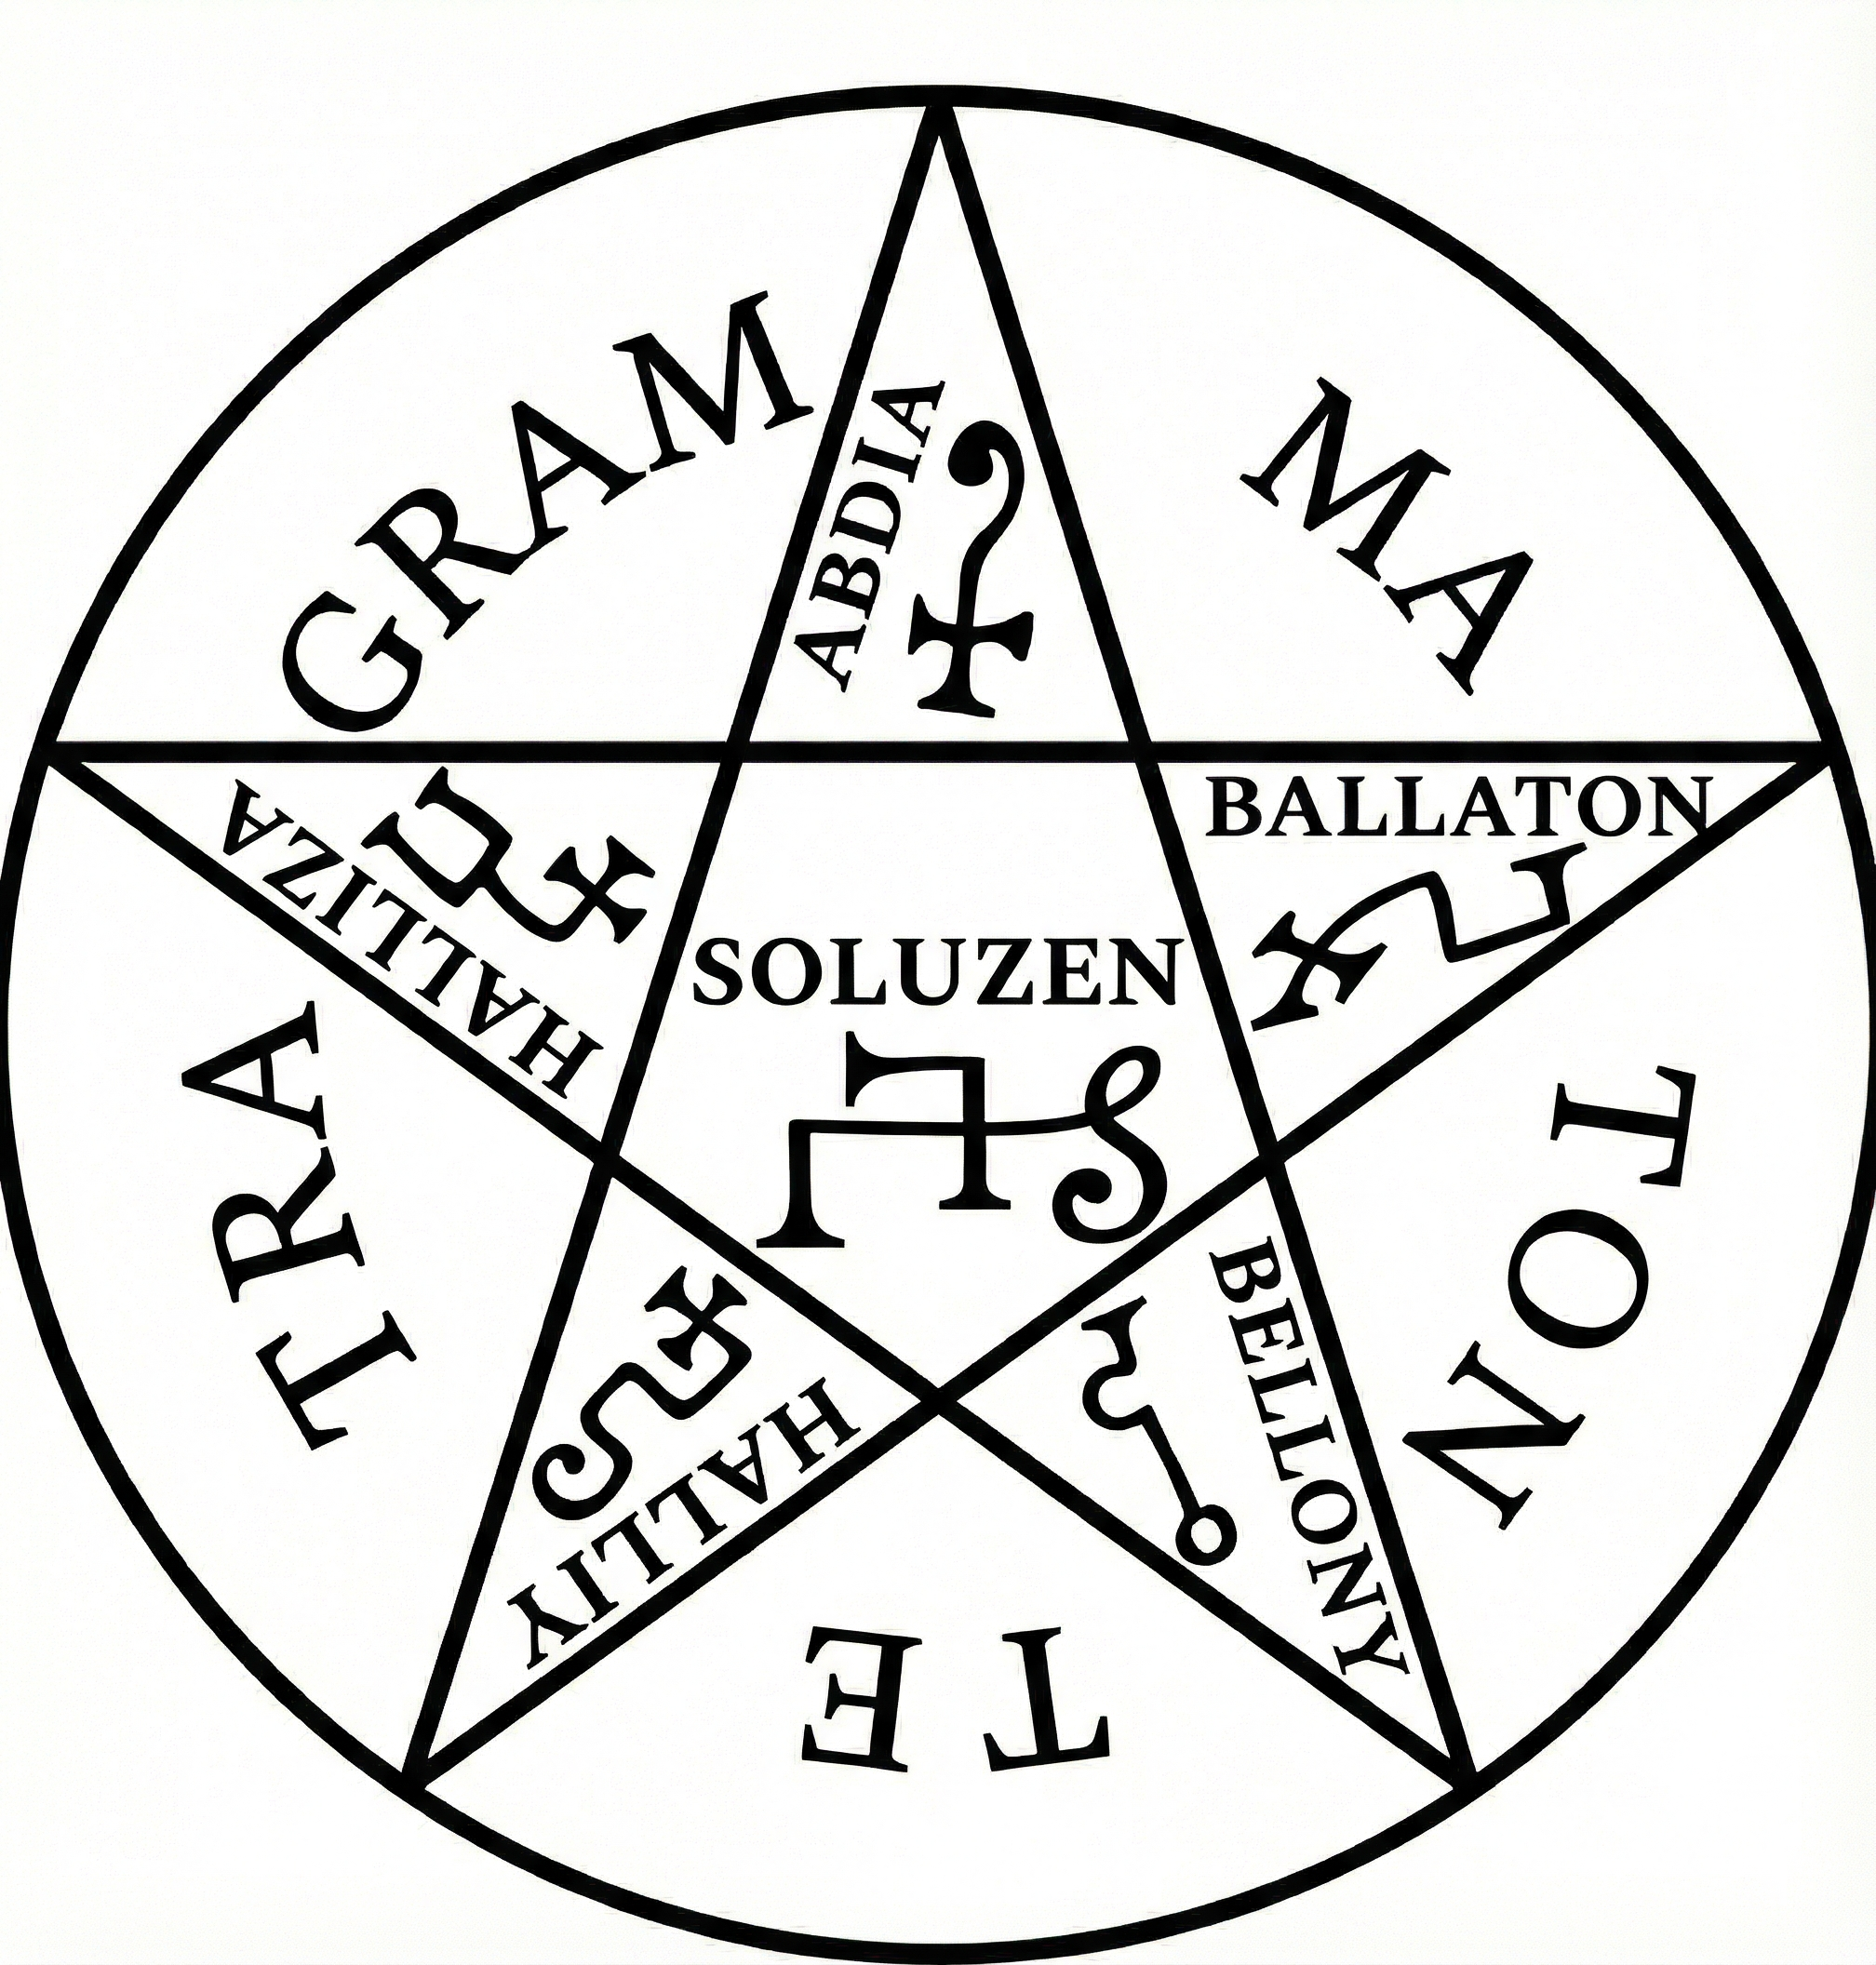
\includegraphics[width=0.3\paperwidth,keepaspectratio]{solomon_pentagram.png}
	\caption{The Pentagram of Solomon}
	\label{fig:solomonpentagram}
	\cite{peterson2001}
\end{figure}
\textbf{Elements:}
\begin{itemize}
	\item Five points: The letters Y-H-Sh-V-H (Yeheshuah, the "Pentagrammaton"—five-letter divine name)
	\item Center pentagon: The letters spelling TETRAGRAMMATON arranged in geometric form
	\item Outer ring: ABDIA, BALLATON, BELLONY, HALLIY, HALLIZA, SOLUZEN (guardian angel names from the Lemegeton tradition)
\end{itemize}
\textbf{Why It's Generalized:}

The pentagram contains no specific entity sigil, no individual demon's seal. It asserts pure authority through divine names and angelic guardians. Any of the 72 spirits will recognize this symbol and respond to it regardless of their individual nature.

\textbf{Practical Use:}

\begin{itemize}
	\item Inscribe on metal (traditionally copper or silver, though any conductive metal suffices)
	\item Wear as pendant during any protective or exorcistic work
	\item Mount above doorways as permanent installation
	\item Draw in air with wand or blade when immediate protection is needed
\end{itemize}

When worn, the pentagram establishes the operator as an agent of the divine authority it represents. This is not symbolic—the texts treat it as a functional tool that alters the operator's position in the spiritual hierarchy.
\subsection{Combined Configuration}
\paragraph{}{The complete defensive architecture combines Circle and Triangle. The operator stands within the Circle (protected space). The Triangle is positioned outside the Circle with its point facing outward, creating a buffer zone.}
\begin{figure}[H]
	\centering
	\includegraphics[width=0.3\paperwidth,keepaspectratio]{solomon_circle_and_triangle.png}
	\caption{Circle and Triangle Combined}
	\label{fig:circletriangle}
\end{figure}

This configuration appears in the Lemegeton as the standard setup for spirit evocation. In that context, the spirit is constrained to appear within the Triangle while the magician remains safe in the Circle. For defensive work, the principle reverses: any intrusive entity approaching the protected space encounters the Triangle's resistance before reaching the Circle's absolute boundary.

\textbf{When to Use:}

\begin{itemize}
	\item Formal defensive ritual in a prepared space
	\item When maximum protection is required
	\item When dealing with known persistent intrusion
	\item As permanent installation in a dedicated working area
\end{itemize}

For emergency or field use, simplified versions suffice (see Emergency Procedures, Appendix).
\subsection{Activation Formula}
\paragraph{}{The geometry and names are inert until spoken. The formula activates the defensive architecture by asserting the operator's authority.
}
\textbf{Standard Banishment:}

\begin{quotation}
	\enquote{By TETRAGRAMMATON, ADONAI, AGLA, ON, EL—depart from this place. By PRIMEUMATON who commands thy beginning and ANAPHAXETON who binds thy form—return to the depths appointed unto thee. By the power of the divine names here inscribed, by the authority of the Circle that cannot be crossed, by the force of the Triangle that drives thee hence—I command thee: BE GONE.}
\end{quotation}

Speak with conviction. The words are not petition—they are declaration. The entity must recognize the authority being invoked, and that recognition is what compels obedience.
